\documentclass[12pt,oneside,openright]{report}

\usepackage[utf8]{inputenc}
\usepackage[scaled]{helvet}

\renewcommand\familydefault{\sfdefault} 
\usepackage[T1]{fontenc}
\usepackage{fancyhdr,xcolor}

\usepackage{graphicx} % Add the graphicx package for including images
\usepackage{geometry}
\usepackage{amsmath} % Add this line to your LaTeX preamble to use \text
\usepackage{afterpage}
\usepackage{caption}
\usepackage{float}
\usepackage{xcolor}
\usepackage[style=authoryear,backend=biber]{biblatex}
\addbibresource{bibliog.bib}
\usepackage[colorlinks=true,linkcolor=black,anchorcolor=black,citecolor=black,filecolor=black,menucolor=black,runcolor=black,urlcolor=black]{hyperref}\usepackage{graphicx}
\geometry{
  a4paper,
  left=20mm,
  right=20mm,
  top=4.5cm,
  headheight=4cm,
  bottom=3.5cm,
  footskip=3cm
}

\renewcommand*{\bibfont}{\footnotesize}

\newcommand{\changefont}{
    \fontsize{18}{16}\selectfont
}
\definecolor{boxcl}{HTML}{1188BB}
\definecolor{tubred}{HTML}{1188BB}



\begin{document}

\begin{titlepage}
    \centering
    % Include the image with a width of one-third of the page
    
\includegraphics[width=0.5\textwidth]{Hu-logo.png}
    \vspace{2cm}
    
    {\huge \textbf{Multisensory Integration in Virtual Reality: Effect of Passive Haptic Stimulation}\par}
    \vspace{2cm}
    {\LARGE Master Thesis\par}
    \vspace{0.5cm}
    {\textbf{submitted in fulfillment of the requirements for the degree}\par}
    Master of Science (M.Sc.)\par
    {\textbf{in the master's program ``Mind and Brain''}\par}
    \vspace{1.5cm}
    {\textbf{Humboldt-Universität zu Berlin}\par}
    {\textbf{Berlin School of Mind and Brain}\par}
    \vfill
    \raggedright
    \begin{tabular}{ll}
        \textbf{Handed in by}: & Benjamin Dupré \\
        \textbf{Date of birth:} & 26.04.1986\\
       \textbf{ Address:} & Hoppestraße 16, 13409, Berlin \\
    \end{tabular}
    \vfill
    \begin{tabular}{ll}
        \textbf{1. Supervisor:}& Professor Dr. Arno Villringer \\
        \textbf{2. Supervisor:}& Dr. Michael Gaebler  \\
    \end{tabular}
    \vfill
    {Berlin, den \today \par}
\end{titlepage}

\section*{Introduction}
\subsection*{Problem \& Significance}

Since the bigginging, research in interoception has shown that visceral signals can influence how we process exteroceptive information. Specific brain mechanisms responsible for predicting signals from within the body, including interoceptive body changes related to heart systole, play a role in diminishing the perception of external body signals, such as touch, vision, and auditory stimuli \parencite{esra_p, AL2021118247, Grund643, motyka, Park2014}. This phenomenon has been well-established in the context psychophysical experimetal set-ups and individual sense modalities.

After that, efforts to integrate findings into more task-relevant information have been carried out. Evidence suggest that more eye movement is generated during the systolic phase of the cardiac cycle and more fixation during the diastolic phase \parencite{GalvezPol2018ActiveSI}. Thus, implying that interoceptive and exteroceptive processing do adjust to each other; inour case, by sampling the outer environment more during quiet periods of the inner organism.

And recently efforts in the direction of The multisensory integration experiment conducted by Saltafossi found that MISSING \parencite{SALTAFOSSI2023108642}. This study examines the influence of the cardiac phase on multisensory integration, a cognitive process that facilitates the nonlinear fusion of sensory input to reduce environmental uncertainty.

As the connection between the heart cycle and perceptual modulation becomes more established, research delves into theoretical explanations. One such explanation is an interoceptive predictive coding process. For example, a recent stuy \parencite{Allen2022}using a Markov decision process (MDP) -- a probabilistic generative model that utilizes the current cardiac cycle and visual stimuli-- shows that the observed phenomena could be explained with this computational model. This model is important because they provide a framework to test or disprove empirical research that could account for psychiatric diseases using computational phenotyping. 

As the heart-coupling modulation research moves further into theoretical generalizations or practical applications the risks associated generating them with not suffucient ecological validated evidence increases.Bringing experiments closer to ecological validity is relevant because it helps us distinguish what is relevant for observed behavior and cognition in the real world. It often refers to the relationship between real-world phenomena and the investigation of these phenomena \parencite{schmuckler2001ecological}. Otherwise, we run the risk of not truly understanding how body-brain phenomena translate into our human psychology.

A tool that can facilitate a smooth transition between psychophysics findings and psychological phenomena is Immersive Virtual Reality (IVR). IVR has proven to be a powerful tool for investigating cognitive processes as it enables researchers to assess behaviors and mental states in complex yet highly controlled scenarios. Traditionally, IVR has relied primarily on visual displays and head-hand movement tracking to create mediated experiences. However, the utilization of VR head-mounted displays in combination with ECG and haptic devices presents new challenges, both in practical and technical terms, and in terms of how it aligns with existing literature \parencite{Klotzsche2023}.-X-X-X TAKE OUT ??? Virtual Reality can help us reverse-engineer the process, starting from what we know are incorrect assumptions and attempting to elucidate if the described mechanisms are triggered. To do this, we first need to validate the experimental setup by replicating the multisensory findings obtained thus far.

Notably, this research seeks to work as a proof of concept by validating an experimental Virual Reality set-up that could take further this two lines of research. Multsisensory modulation and effects in environment sampling of cardiac cycle. Thus, bringing this findings closer to ecological validity and everyday life. However, accurately assessing the extent to which this phenomenon influences everyday experiences, such as how we feel after running, is challenging. It requires a delicate balance between obtaining clear psychophysical results and integrating them with other cognitive functions.

\subsection*{Thesis Topic \& Goal}

The primary objective of this study is to investigate the feasibility of incorporating touch-cardiac-cycle modulation studies into Interactive Virtual Reality (IVR) setups. IVR, being a system that often involves visual, tactile, and proprioceptive senses, inherently engages multiple senses or is intentionally designed as a multisensory experience. To facilitate a comparative analysis of results, a relevant recent study by Martina Saltafossi on vision, touch, and hearing as multisensory pairs \cite{SALTAFOSSI2023108642} serves as a suitable reference. While there is limited research on two multisensory modalities and none to my knowledge using IVR, this study aims to bridge that gap. However, before delving into specific goals, it is necessary to define the concept of touch, as it encompasses various modes.

The extended classification of tactile sensation \cite{Healy2003HandbookOP} provides a useful framework for understanding touch, categorizing it into five different modes based on the presence or absence of voluntary movement: (1) tactile (cutaneous) perception, (2) passive kinesthetic perception, (3) passive haptic perception, (4) active kinesthetic perception, and (5) active haptic perception. For this thesis, touch is defined as passive haptic perception generated by a vibrating Data-Glove. Based on this definition, three main goals are derived:

\begin{itemize}
  \item[(i)] Assess the impact of passive haptic stimuli on the reported sense of immersion in individuals. This investigation aims to quantify the extent to which passive haptic stimuli influence overall reported scores in questionnaires, shedding light on the role of touch in creating a sense of presence. Saltafossi's study refers to this as "body illusions induced by multisensory conflicts between exteroceptive sensory modalities, such as vision and touch."
    
  \item[(ii)] Confirm the findings supporting the redundancy signal effect (RSE). This means that bimodal stimulations have a faster response time (RT) than unimodal. In this case, it refers to 2 combinations ($V/(V=T)$, $V/(V\neq T)$) Were unimodal is visual and bimodal is visual and touch. Touch can be matchin visual or not matching visual space. Considering also grossly Race model (RMI)inequality findings concerning with significant differences between conditions. 
\end{itemize}

By examining how passive haptic stimuli influence the response time in the motor-memory task, this study seeks to replicate the overall findings of the reference paper \parencite*{SALTAFOSSI2023108642} and validate behaviorally the effects of passive haptic stimuli in a IVR motor-memory task. 

Through an investigation of passive haptic touch's influence on immersion, behavioral outcomes, and interactions with the cardiac cycle, this research aims to enhance our understanding of IVR as a research tool and further validate findings on multisensory integration and perception.


\section*{Methods}
    \subsection*{Participants}
    From an original pool of 23 participants that presneted to do the task we finish we 20 participats. Two of them did not fill all questionnaires and a third one was above the age limit  so we had to exclude them from the analysis, leaving us with 20 participants. The call for participants was answered considerably more by women (15) than men (5). The age across the sample was consistently around 25 years old, with the exception of one participant ($\mu=25.1 , \sigma=6.3$).
    \begin{figure}[h]
        \centering
        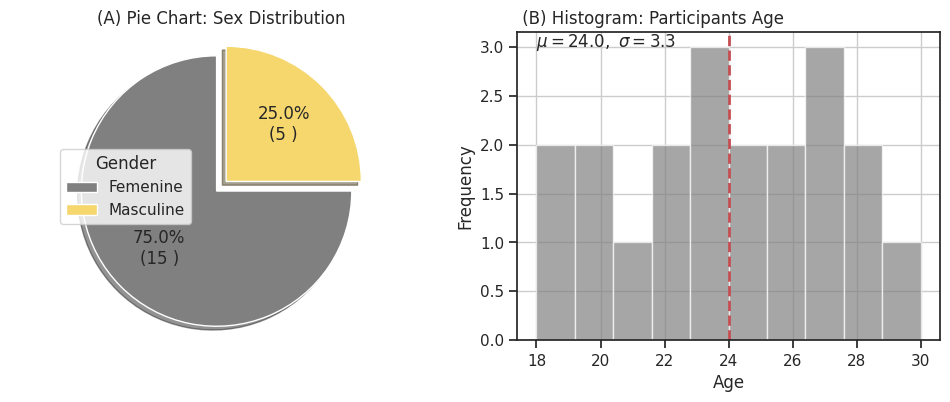
\includegraphics[width=12cm]{/home/perdices/Dokumente/Github/m-b_thesis/Analysis/figures/participants.png}
        \caption{Participants Composition}
        \label{fig:mesh1}
    \end{figure}
    
    \subsection*{Materials}
    \subsubsection*{3.2.1 Electrocardiogram (ECG):}
Heart rate data is collected using an Arduino Uno and a SparkFun Single Lead Heart Rate Monitor - AD8232. The collected data is transferred through a USB 2.0 connection and integrated into the Unity log file at a frequency of 133 Hz. Based on live ECG device \parencite{TimsECG}.

\subsubsection*{3.2.2 Head Mounted Display \& Lighthouses:}
The VR setup includes an HTC Vive head-mounted display (HMD) with two lighthouses. The headset specifications include a Dual AMOLED 3.6" diagonal display, with 1080 x 1200 pixels per eye (2160 x 1200 pixels combined), a 90 Hz refresh rate, and a 110-degree field of view. The lighthouses are equipped with SteamVR Tracking, G-sensors, gyroscopes, and proximity sensors. Both the HMD and lighthouses are connected using USB 2.0. For this study, the VR controllers were not used, and instead, hand tracking was performed using the Leap Motion sensor.

\subsubsection*{3.2.3 Leap Motion Controller:}
The Leap Motion Controller has a field of view of 150x120 degrees, with a variable range of roughly 80 cm (arm's length). It weighs 32 grams and is mounted on the HMD. The device features two 640x240 infrared cameras with a frame rate of 120 fps.

\subsubsection*{3.2.4 Data Gloves:}
The data gloves used in the study are equipped with magnetic sensors and connected to Unity using a microUSB connection. These gloves provide haptic feedback through 10 vibrotactile actuators, offering a wide range of tactile sensations with 1,024 levels of intensity. The gloves also incorporate complete finger tracking using six 9-axis Inertial Measurement Units (IMUs). These IMUs enable precise tracking of finger movements, allowing for accurate gesture recognition and enhanced interaction in virtual environments.
    \subsection*{Task}
    After being debriefed and receiving information about the experiment, participants completed the following tasks:
\begin{enumerate}
\item[(i)] Edinburgh Handedness Questionnaire
\item[(ii)] PRE-Cybersickness Questionnaire
\end{enumerate}

Following the completion of the first set of questionnaires, the participants were taken to another room where the IVR (Immersive Virtual Reality) equipment was set up. This equipment included a head-mounted display (HMD), data gloves, and an ECG (Electrocardiogram) device. Participants underwent a short training session before proceeding with the heartbeat count task and the IVR memory-motor task.

\begin{enumerate}
\item[(iii)] PRE-Heart Beat Count Task (HCT) for one minute. (This task is not considered in this thesis.)
\item[(iv)] IVR Memory-Motor Task: In this environment, participants were positioned in front of a virtual table and given sufficient time to acclimate to the virtual surroundings. A sketch of a puzzle was displayed in front of the virtual room, which they needed to memorize. During the memorization phase, participants kept their virtual hands open with palms facing up. Subsequently, the sketch disappeared from their visual field, and a red ball was introduced from the top, appearing in either one of the hands. Participants observed a template on the table, which was an identical representation of the initial sketch they had memorized. Their task was to place the ball in the correct location on the template as quickly as possible. Throughout 108 trials, three different conditions (relevant haptic stimuli, irrelevant haptic stimuli, and no haptic stimuli) were randomly presented an equal number of times (36 times each). The trials appeared rapidly, one after the other. The start of each trial was marked by placing the ball in a hand, and the end of the trial was marked by the moment the ball reached the designated location on the template.
\item[(v)] POST-Heart Beat Count Task (HCT) for one minute. (This task is not considered in this thesis.)
\end{enumerate}

The final step of the experiment involved two questionnaires aimed at extracting information on several relevant fields for the goal of this thesis:
After the IVR part the participants filled a again the cybersicknesss quiestionaire as well as for the first time an overall Subjective Evaluation Questionaire.
\begin{enumerate}
    \item[(vi)] Virtual Reality Subjective Evaluation Questionnaire
    \item[(vii)] POST-Cybersickness Questionnaire
\end{enumerate}
    \subsection*{Mesurements}
    \subsubsection*{Immersive Virtual Reality (VR):}

The VR experience was presented and tracked using an HTC Vive head-mounted display (HMD), two lighthouses, a Leap Motion sensor, and Haptic Data Gloves. Movement data from the data gloves, Leap Motion device, and the HMD was collected. For movement analysis, only the wrist movements tracked by the Leap Motion device were considered, excluding the fingertips' magnetic tracking sensor data. All movements were recorded in a Euclidean coordinate system (X, Y, Z) with the original calibrating point set at (0, 0, 0). This provided a total of nine streaming sources of data (e.g., Headset X, Headset Y, Headset Z, and so on). Notably, rotational data was not included in the analysis.

Additionally, in the game output data, there are flags that signal if a button was pressed, if the ball is placed in the holder, and when the trial started.

\subsubsection*{Electrocardiogram (ECG):}

Heart rate data was collected using a USB cable and integrated into Unity Engine. This information was coupled with all other Unity data at a frequency of 133 Hz.

\subsubsection*{Questionnaires:}

\begin{enumerate}
\item[(i)] Virtual Reality Subjective Evaluation Questionnaire: This self-made questionnaire consists of 26 items oriented towards capturing whether the VR experience felt real for the participant or not. It explores the level of engagement, hand movement, task difficulty, and other controlling factors. The questionnaire uses a Likert scale ranging from one to seven.
\item[(ii)] PRE/POST-Cybersickness Questionnaire: The version applied in this study is a shorter adaptation of the simulator sickness questionnaire (SSQ) \parencite*{avpsy}. It employs a Likert scale ranging from one to four, with labels going from "not present," "somewhat," "clearly," and "very strongly." The questionnaire includes 16 items based on symptoms, such as "fatigue" and "general discomfort," among others.
\end{enumerate}
    \subsection*{Data Analysis}
    \section*{Results}
    \subsection*{(i) Assessing the Impact of the Haptic Globe on Reported Immersion}
    
    Nineteen respondents answered 27 questions, rating them on a scale from 1 (Does Not Apply) to 7 (Totally Applies). The key findings from the questionnaire are as follows:
    
    \begin{enumerate}
        \item In question number 24, the perceived increase in immersion due to the haptic globes was high ($\text{Mdn} = 6$, $\mu = 6$, $\sigma = 0.76$). Furthermore, the task was considered enjoyable at least some of the time ($\text{Mdn} = 6$, $\mu = 5.4$, $\sigma = 1.04$).
        
        \item Question 26 revealed that haptic feedback was perceived as either not significantly improving performance or having a neutral effect ($\text{Mdn} = 3$, $\mu = 3.6$, $\sigma = 1.49$). Similarly, in question 12, the perception of haptic feedback improving response time was generally rated as neutral to not applicalbe ($\text{Mdn} = 3$, $\mu = 3.7$, $\sigma = 1.74$). In question 7, when asked about the impact on results, haptic feedback was perceived as not applicable ($\text{Mdn} = 6$, $\mu = 6$, $\sigma = 0.76$).
    
        \item Notably, the assertion that it was very challenging to remember the position of the red ball ($\text{Mdn} = 2$, $\mu = 2.9$, $\sigma = 1.45$) was generally disagreed upon. Conversely, in question 8, which asked about the ease of remembering the location of the red ball, responses were as expected ($\text{Mdn} = 5$, $\mu = 5.1$, $\sigma = 1.37$).
    
        \item The highest variance was observed in question 13 ($\text{Mdn} = 5$, $\mu = 4.2$, $\sigma = 1.79$), indicating that haptic feedback made it easier to place the ball. Similarly, question 18, which inquired about the ease of counting heartbeats at the beginning of the experiment, also showed significant variance ($\text{Mdn} = 4$, $\mu = 4$, $\sigma = 1.79$). 
        
    \end{enumerate}
    
    For more details please go to the supplement section 

    
    \subsection*{(ii) Touch stimuli influence the response time}
\section*{Discussion}


%-------- CREATING BIBLIOGRAPHY

%\bibliographystyle{plain} % Choose your style
%\bibliography{bibliog.bib}  % Use your actual .bib file name
\pagebreak
\section*{Supplement}
    \begin{figure}[H]
        \centering
        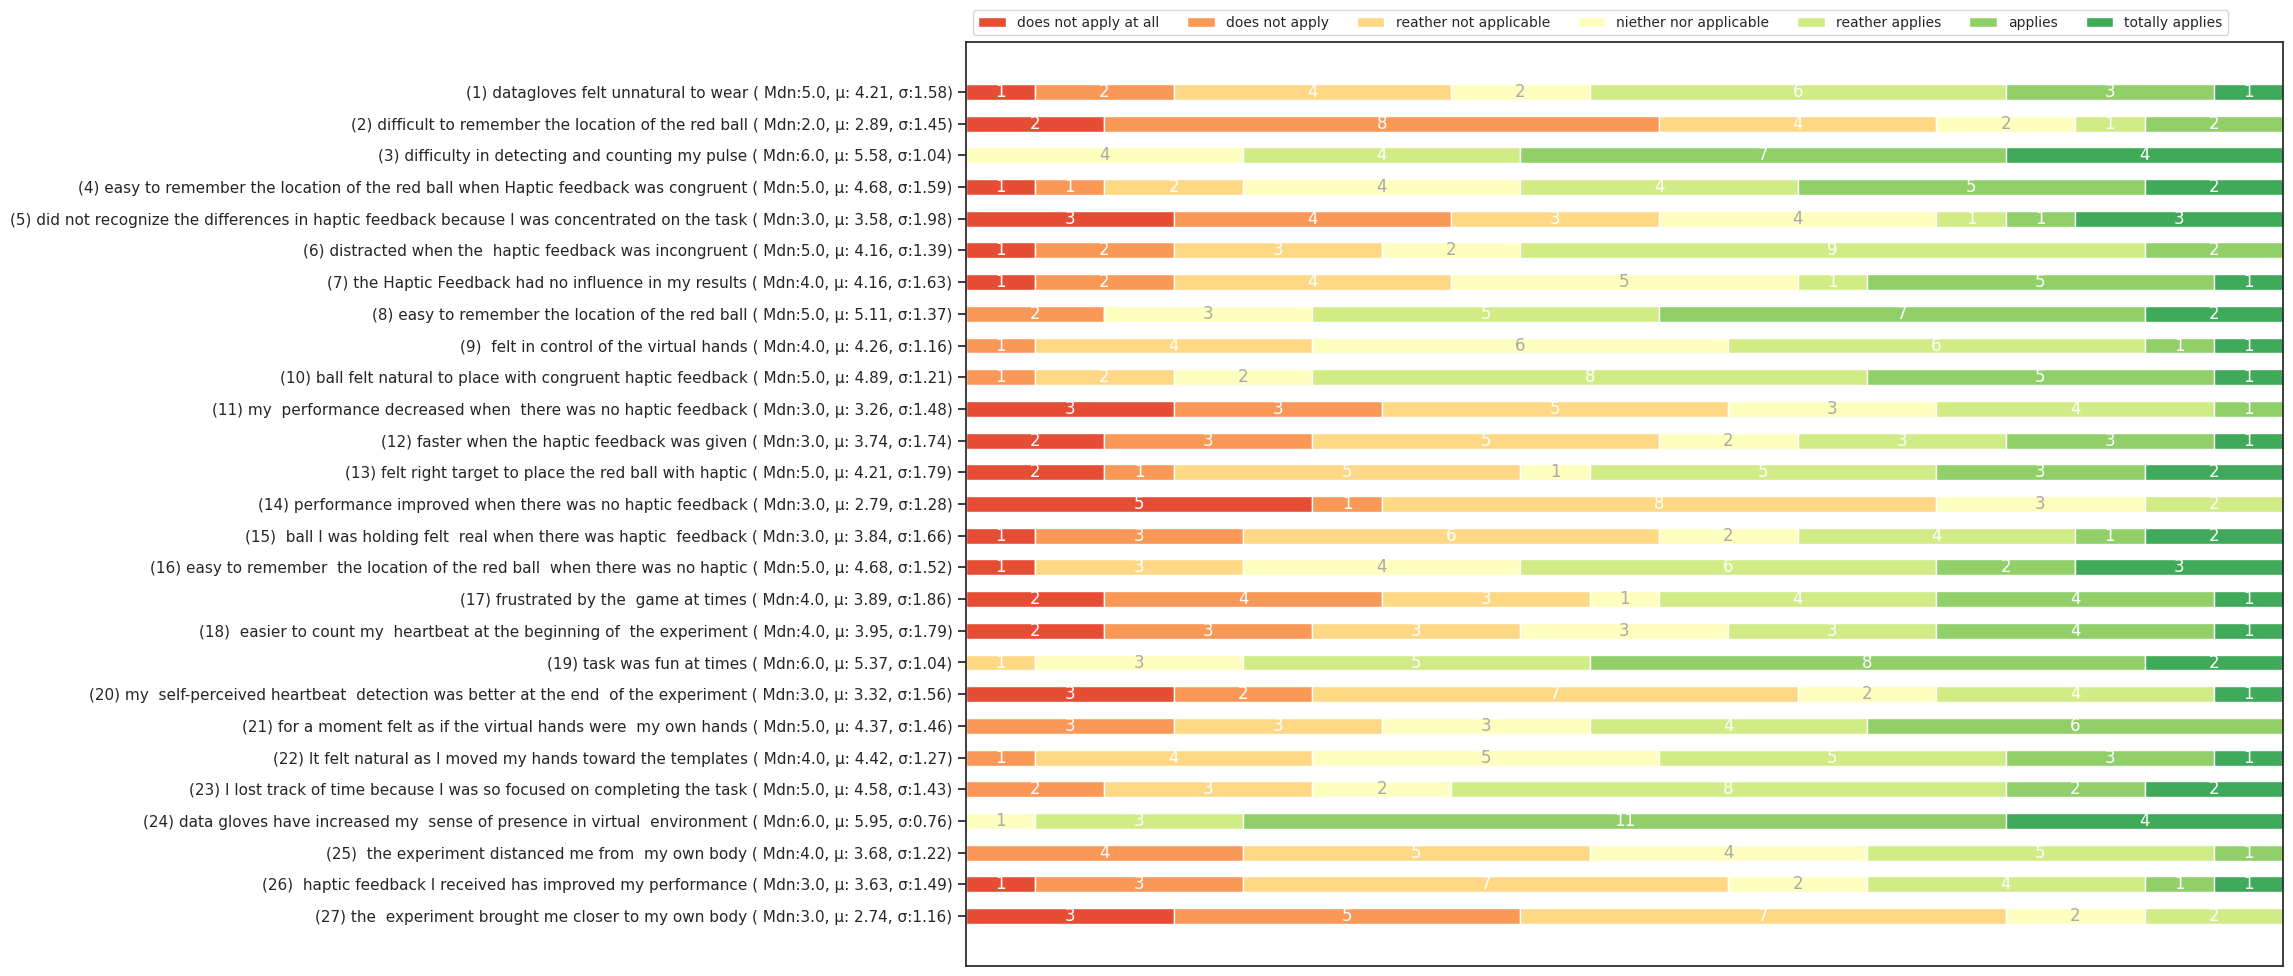
\includegraphics[angle=90, width=\textwidth, height=20cm, keepaspectratio]{/home/perdices/Dokumente/Github/m-b_thesis/Analysis/figures/questionaire_fig.png}
        \caption{Results: Virtual Reality Subjective Evaluation Questionnaire}
        \label{fig:mesh2}
    \end{figure}
  

\pagebreak
\paragraph{\textbf{References}}
\printbibliography[heading=none]

\end{document}

